Consider more general case Fig. \ref{38f}.

\begin{figure}[h]
\centering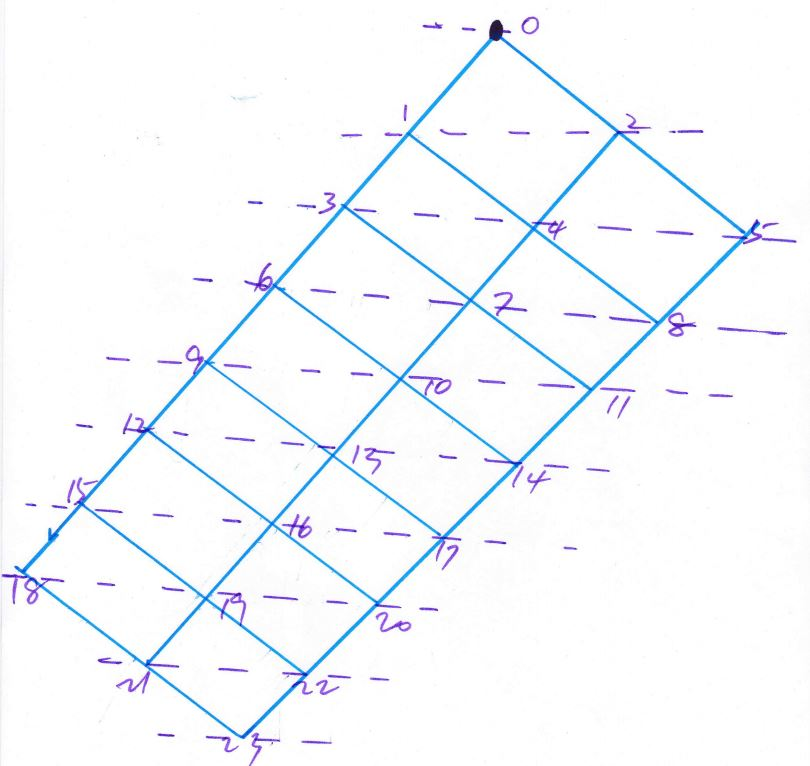
\includegraphics[width=0.7\linewidth]{figure/c38_f}
\caption{3*n $n = 8$ regular mesh}
\label{38f}
\end{figure}

The closed formula groups are presented as following:

\begin{equation}
{
\left[ \begin{array}{cccccccccc}
1 & 2 & 3 & 3 & 3 & 3 & 3 & 3 & 2 & 1\\
1 & -1 & 0 & 0 & 0 & 0 & 0 & 0 & 0 & 0\\
0 & \sigma-1 & 1 & 0 & 0 & 0 & 0 & 0 & 0 & 0 \\
0 & \sigma-1 & \sigma & 1 & 0 & 0 & 0 & 0 & 0 & 0 \\
0 & \sigma-1 & \sigma & \sigma & 1 & 0 & 0 & 0 & 0 & 0\\
0 & \sigma-1 & \sigma & \sigma & \sigma & 1 & 0 & 0 & 0 & 0\\
0 & \sigma-1 & \sigma & \sigma & \sigma & \sigma & 1 & 0 & 0 & 0\\
0 & \sigma-1 & \sigma & \sigma & \sigma & \sigma & \sigma & 1 & 0 & 0\\
0 & \sigma-1 & \sigma & \sigma & \sigma & \sigma & \sigma & \sigma & 1 & 0\\
0 & \sigma-1 & \sigma & \sigma & \sigma & \sigma & \sigma & \sigma & \sigma & 1 \\
\end{array} 
\right ]} \times \left[ \begin{array}{c}
\alpha_{0} \\
\alpha_{1} \\
\alpha_{3} \\
\alpha_{6} \\
\alpha_{9} \\
\alpha_{12}\\
\alpha_{15}\\
\alpha_{18}\\
\alpha_{21}\\
\alpha_{23}
\end{array} 
\right ] = \left[ \begin{array}{c}
1 \\
0 \\
0 \\
0 \\
\vdots \\
0
\end{array} 
\right ]
\end{equation}
